
\chapter{The Smart Grid Control System}


\section{Introduction}

Analogous with the modernisation of the classic \acrlong{pg} into the \acrlong{sg}, the \acrshort{scada} subsystem of the \acrshort{pg} is the predecessor of the control system of the modern \acrlong{sg}.
Therefore, a description of the \acrshort{scada} system, evolving from the centralised subsystem controlling the Classic \acrshort{pg}, to the modernised verion of the \acrshort{scada} subsystem, initiates the description of the \acrlong{sg} Control System. 



 
   \begin{figure}[ht]

    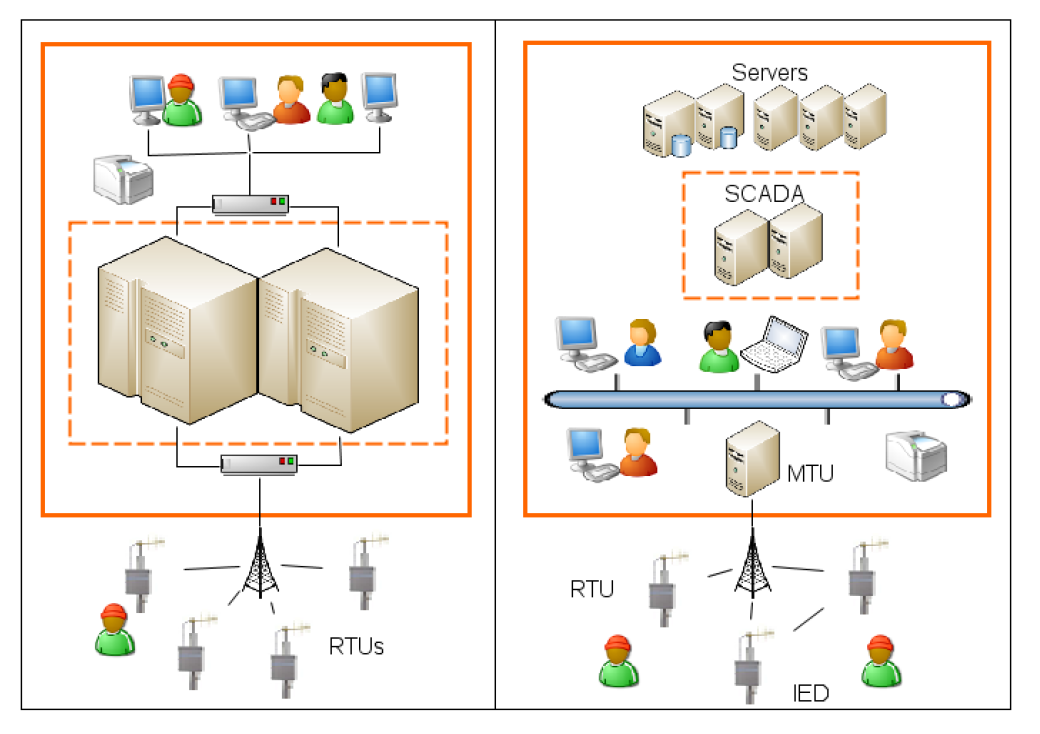
\includegraphics[width=\textwidth]{figures/SCADA-CentralisedAndDistributed.png}    


\caption[A Centralised and Distributed SCADA system]{A Centralised and Distributed SCADA system \cite[p. 123]{alcaraz2012security}}
\label{fig:SCADA-CentralisedAndDistributed}
\end{figure}



The characteristics of the three generations of SCADA systems described by \Citeauthor{alcaraz2012security} in \cite{alcaraz2012security}, may be summarised below:
 

 \begin{enumerate}
     \item A Monolithic SCADA system utilises a centralised offline control center  infrastructure, in order to monitor and control the physical system by proprietary control mechanisms.
     \item A Distributed SCADA system utilises a networked, but centralised control  center in order to monitor and control the physical system by proprietary control mechanisms. 
     \item A Networked SCADA system utilises a networked, and online control  center in order to monitor and control the physical system by standardised control mechanisms.
 \end{enumerate}



 \begin{figure}[ht]
\centering
    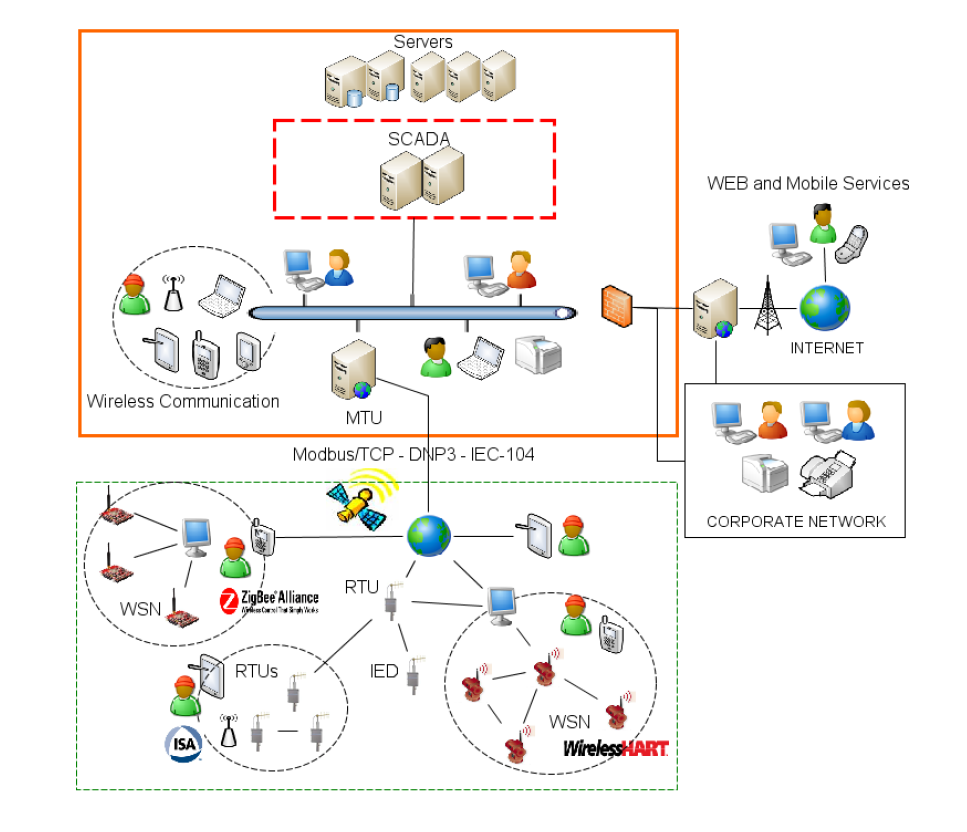
\includegraphics[trim=20 20 20 10, clip, width=\textwidth]{figures/SCADA-Current.png}
\caption[A Current SCADA system]{A Current SCADA system \cite[p. 124]{alcaraz2012security}}

\end{figure}





\subsection{The Modernised SCADA system}
 
 The \acrshort{scada} system is, as described in \cite{alcaraz2012security}, a system utilised to supervise and control \acrfull{ci} systems, including \acrshort{pg} infrastructures. Initially designed in order to control physical infrastructure systems like the classic \acrlong{pg}, the Monolithic SCADA system emerged into the Distributed SCADA system. The transition from a Monolithic SCADA system to a Distributed SCADA system transforms, as indicated by figure \ref{fig:SCADA-CentralisedAndDistributed}, the central management center from a centrally controlled mainframe environment, to a networked server environment controlled by operators connected through a \acrfull{lan}
  
  
 The \acrshort{sg} control center emerged from the Distributed SCADA system, into the Networked SCADA system used in order to control modern \acrlong{cps}s, like the \acrshort{sg}.\\ 
 


 





 




However, as explained by \Citeauthor{zamani2020introduction} in \Cite{zamani2020introduction}, the \acrshort{scada} system has a number of shortcomings, making it unsuitable for a \acrshort{sg} enegy distribution monitoring system:

\begin{itemize}
    \item The data polling rate is once every 2-10s, which is not sufficient in order to get real-time measurements.
    \item No time-stamps are attached to samples, making it hard to monitor rate of change over time
    \item State Estimation is not performed with sufficient frequency, if at all.
    \item The ability to observe dynamics is not supported by the system.
\end{itemize}





In order to address these shortcomings, the \acrfull{wams} system\footnote{WAMS is also known as the Wide Area \textbf{Monitoring} System}, described next, was invented.






\subsection{Smart Grid  Control system}
The \acrlong{sg} system constitutes a complex system of subsystems, which proper operation is a prerequisite for the successful transmission of electric energy from producers to consumers, according to the current demand for energy, as controlled by the Demand Management system, dynamically adjusting the energy supply accordingly. In order to successfully reply to the dynamically changing demands for energy, a close monitoring of the production and transmission of energy through the Wide Area network is required. \\ 

The \acrshort{sg} consists of a vast number of both conventional and modern, more dynamic, production facilities, which requires thorough monitoring in order to ensure the optimal distribution of electrical energy. The requirement of a consistently stable and reliable supply of energy is constant, while the amount of energy demanded is dynamically changing according to the demand for power at any time. \\ 

Therefore, the proper \acrshort{sg} operation might be considered virtually impossible without a  close monitoring of current power flow, as well as the ability to instantly adjust the supply of power according to present needs,  without the risk of causing power surges or blackouts. For this purpose, the Wide Area Monitoring System analyses the levels of electrical power as monitored by sensors, synchronised according to a common GPS-controlled time source. \\ 

The correctness of this time source is critical to the reliability, and therefore, the proper operation of the monitoring system, constituting the primary decision criteria for actions controlling the supply of power.





\section{WAMS state estimation}
In order to monitor 


